% Phân tích chuyên sâu (3): từng nước và thống kê ván đấu. \input trong 04-thuc-nghiem.tex.
\section{Phân tích từng nước trên 2.800 ván}
\label{sec:cs-tung-nuoc}
Bộ chiến thuật đo trên thế chọn sẵn. Mục này đo trong ván thật: mọi nước sau khai cuộc của RR8 giữ riêng, tổng 56\,688
nước, được gắn tối đa một nhãn theo thứ tự ưu tiên: bỏ lỡ nước thắng ngay; bỏ sót chặn ô thắng duy nhất; thế đã thua
(đối thủ có hai ô thắng); bỏ lỡ VCF; và cuối cùng, ở thế yên tĩnh, ``để hở VCF'' khi còn nước an toàn mà vẫn chọn
nước cho đối thủ một VCF. Hai loại cuối dùng trọng tài VCF nên là cận dưới.

\subsection{Lỗi theo tác tử}
\begin{table}[H]
  \centering
  \footnotesize
  \caption{Lỗi chiến thuật từng nước trong 2.800 ván RR8 giữ riêng}
  \label{tab:cs-nuoc-loi}
  \begin{tabular}{lrrrrrr}
    \toprule
    Tác tử & Nước & Bỏ thắng & Sót chặn & Bỏ VCF & Để hở VCF & Lỗi/100 \\
    \midrule
    L1 Random & 3.553 & 56/57 & 120/122 & 133/137 & 847/2421 & 32,54 \\
    L2 Rule & 7.094 & 0/313 & 0/1053 & 42/384 & 293/4941 & 4,72 \\
    L3 AlphaBeta & 9.028 & 0/398 & 0/1031 & 59/615 & 97/6693 & 1,73 \\
    L4 MCTS & 3.727 & 253/352 & 66/73 & 358/433 & 636/2280 & 35,23 \\
    L5 PolicySL & 7.544 & 60/408 & 0/912 & 26/558 & 173/5329 & 3,43 \\
    L6 PolicyRL & 8.389 & 14/422 & 20/1163 & 34/610 & 191/5925 & 3,09 \\
    L7 PUCT & 8.300 & 23/586 & 21/1064 & 59/922 & 72/5635 & 2,11 \\
    L8 AlphaZero & 9.053 & 1/603 & 10/1344 & 64/978 & 41/6063 & 1,28 \\
    \bottomrule
  \end{tabular}
  \par\smallskip\parbox{.95\linewidth}{\footnotesize Mẫu số của mỗi cột là số lượt mà tình huống đó xuất hiện. ``Để hở VCF'': không có đường thắng ép, còn nước an toàn nhưng chọn nước cho đối thủ có VCF; mẫu số là mọi lượt yên tĩnh.}
\end{table}

Đọc Bảng~\ref{tab:cs-nuoc-loi} theo cột:
\begin{itemize}
  \item \textbf{Bỏ thắng ngay.} L2 và L3 bằng 0 nhờ luật P1 và nước bắt buộc. L5 bỏ 60/408 ($14{,}7\%$), khớp với lỗi
  nhãn ở Mục~\ref{sec:cs-du-lieu}. L7 vẫn bỏ 23/586 dù có tìm kiếm: PUCT không có bước kiểm tra nước thắng ở gốc, và
  khi tiên nghiệm của nước thắng thấp trong khi nhiều nước khác cũng thắng sau đó, lượt thăm bị chia.
  \item \textbf{Sót chặn.} L5 không sót lần nào trong 912 tình huống, nhưng L6 sót 20 và L7 sót 21. REINFORCE tinh
  chỉnh policy theo thắng thua và có thể đánh đổi phản xạ chặn học từ expert lấy các nước tấn công.
  \item \textbf{Để hở VCF.} Đây là cột phân biệt các cấp mạnh: L8 $0{,}68\%$, L7 $1{,}28\%$, L3 $1{,}45\%$, L5 và L6 khoảng
  $3{,}2\%$, L2 $5{,}9\%$, MCTS $27{,}9\%$.
  \item \textbf{Bỏ VCF.} L7 và L8 bỏ khoảng $6\%$ cơ hội, cao hơn L5 ($4{,}7\%$): khi có nhiều đường thắng, tìm kiếm có thể
  chọn đường chậm hơn mà không phải đường tứ liên tiếp. Nhãn ``bỏ VCF'' không có nghĩa nước đó làm mất thế thắng.
\end{itemize}
Tổng số lỗi trên 100 nước xếp L8 ($1{,}28$) trước L3 ($1{,}73$), L7 ($2{,}11$), L6, L5, L2 rồi MCTS và ngẫu nhiên. Thứ tự
này gần trùng xếp hạng giải đấu, ngoại trừ L3 đứng trên L7 và L6 về lỗi (và L1 trên L4); riêng L7 mạnh hơn L3 rõ khi đấu: lỗi VCF không đo
được chất lượng nước yên tĩnh, vốn là chỗ mạng giúp L7.

\begin{table}[H]
  \centering
  \small
  \caption{Số lần bỏ lỡ VCF theo độ dài (số nước tấn công)}
  \label{tab:cs-nuoc-vcf}
  \begin{tabular}{lrrrr}
    \toprule
    Tác tử & 2 & 3 & 4 & $\ge 5$ \\
    \midrule
    L1 Random & 92/94 & 22/22 & 11/12 & 8/9 \\
    L2 Rule & 0/294 & 13/37 & 20/35 & 9/18 \\
    L3 AlphaBeta & 0/387 & 1/111 & 21/56 & 37/61 \\
    L4 MCTS & 309/381 & 29/32 & 12/12 & 8/8 \\
    L5 PolicySL & 0/358 & 0/95 & 13/54 & 13/51 \\
    L6 PolicyRL & 0/397 & 6/110 & 8/53 & 20/50 \\
    L7 PUCT & 0/560 & 3/189 & 34/102 & 22/71 \\
    L8 AlphaZero & 1/585 & 11/209 & 23/108 & 29/76 \\
    \bottomrule
  \end{tabular}
\end{table}

\begin{table}[H]
  \centering
  \small
  \caption{Tỷ lệ nước mắc lỗi chiến thuật (\%) theo giai đoạn ván}
  \label{tab:cs-nuoc-giaidoan}
  \begin{tabular}{lrrrrr}
    \toprule
    Tác tử & Nước 1--8 & 9--16 & 17--24 & 25--32 & $\ge 33$ \\
    \midrule
    L1 Random & 27,2 & 24,3 & 47,9 & 61,6 & 53,0 \\
    L2 Rule & 0,0 & 3,2 & 11,4 & 6,5 & 4,7 \\
    L3 AlphaBeta & 0,0 & 0,9 & 4,2 & 2,9 & 1,5 \\
    L4 MCTS & 23,6 & 26,7 & 61,6 & 75,7 & 71,4 \\
    L5 PolicySL & 0,0 & 2,5 & 6,3 & 5,0 & 5,2 \\
    L6 PolicyRL & 0,0 & 1,6 & 5,6 & 8,1 & 3,2 \\
    L7 PUCT & 0,0 & 1,0 & 4,6 & 4,6 & 1,9 \\
    L8 AlphaZero & 0,0 & 0,4 & 2,8 & 1,6 & 1,8 \\
    \bottomrule
  \end{tabular}
\end{table}

Bảng~\ref{tab:cs-nuoc-giaidoan} cho thấy hầu như không có lỗi ở 8 nước đầu với các tác tử có kiến thức, và đỉnh lỗi
rơi vào nước 17--32, giai đoạn các đe doạ dày lên. Với MCTS và ngẫu nhiên, tỷ lệ cao hơn hẳn, tăng mạnh từ nước 17 đến nước 32 rồi giảm nhẹ.

\subsection{Ai tạo được đường thắng ép trước}
\begin{table}[H]
  \centering
  \small
  \caption{Ván mà tác tử là bên đầu tiên có đường thắng ép}
  \label{tab:cs-nuoc-dautien}
  \begin{tabular}{lrrrr}
    \toprule
    Tác tử & Số ván & Thắng (\%) & Nước (trung vị) & Còn lại (trung vị) \\
    \midrule
    L1 Random & 19 & 5,3 & 16 & 14 \\
    L2 Rule & 327 & 94,2 & 8 & 3 \\
    L3 AlphaBeta & 398 & 98,0 & 13 & 3 \\
    L4 MCTS & 81 & 100,0 & 15 & 15 \\
    L5 PolicySL & 356 & 94,7 & 9 & 3 \\
    L6 PolicyRL & 407 & 97,1 & 12 & 3 \\
    L7 PUCT & 557 & 99,6 & 16 & 3 \\
    L8 AlphaZero & 601 & 99,7 & 17 & 3 \\
    \bottomrule
  \end{tabular}
  \par\smallskip\parbox{.95\linewidth}{\footnotesize Đường thắng ép gồm thắng ngay và VCF. ``Còn lại'' là số nước từ lúc đó đến hết ván.}
\end{table}

Bên đầu tiên có đường thắng ép gần như luôn thắng: L7 và L8 chuyển hoá trên $99\%$, L3 $98\%$, L5 và L2 khoảng
$94$--$95\%$. Vì vậy khác biệt sức mạnh chủ yếu nằm ở \emph{ai tạo được đe doạ trước}, thể hiện qua số ván: L8 là bên
đầu tiên trong 601 ván, L2 chỉ 327. MCTS khi tạo được đường thắng thì thắng cả 81 ván nhưng cần trung vị 15 nước để
kết thúc, so với 3 nước của các tác tử khác: rollout không tìm ra nước kết liễu ngắn.

\subsection{Ván kết thúc ra sao}
\begin{table}[H]
  \centering
  \footnotesize
  \caption{Nước cuối cùng của bên thua trong các ván có thắng thua}
  \label{tab:cs-nuoc-ketthuc}
  \begin{tabular}{lrrrrrr}
    \toprule
    Bên thua & Ván & Đòn kép & Sót chặn & Bỏ thắng & Hết nước đỡ & Khác \\
    \midrule
    L1 Random & 699 & 640 & 48 & 11 & 0 & 0 \\
    L2 Rule & 378 & 378 & 0 & 0 & 0 & 0 \\
    L3 AlphaBeta & 270 & 270 & 0 & 0 & 0 & 0 \\
    L4 MCTS & 601 & 573 & 28 & 0 & 0 & 0 \\
    L5 PolicySL & 343 & 336 & 0 & 7 & 0 & 0 \\
    L6 PolicyRL & 267 & 252 & 15 & 0 & 0 & 0 \\
    L7 PUCT & 111 & 92 & 19 & 0 & 0 & 0 \\
    L8 AlphaZero & 63 & 61 & 2 & 0 & 0 & 0 \\
    \bottomrule
  \end{tabular}
  \par\smallskip\parbox{.95\linewidth}{\footnotesize ``Đòn kép'': trước nước cuối của bên thua, đối thủ đã có từ hai ô thắng. ``Sót chặn'': còn một ô thắng mà không chặn. ``Bỏ thắng'': bên thua có nước thắng ngay nhưng đi chỗ khác. ``Hết nước đỡ'': không nước nào ngăn được VCF.}
\end{table}

Hầu hết ván có thắng thua kết thúc bằng đòn kép không đỡ được. Phần ``sót chặn'' nhỏ nhưng khác nhau giữa các cấp:
ngẫu nhiên 48 ván, MCTS 28, L7 19, L6 15, L8 chỉ 2, L2 và L3 không có. Kết hợp với Bảng~\ref{tab:cs-nuoc-loi}: lỗi
quyết định thường xảy ra \emph{trước} nước cuối, lúc bên thua để đối thủ dựng được đòn kép.

\section{Thống kê ván đấu và độ ổn định của xếp hạng}
\label{sec:cs-thong-ke-van}
\subsection{Hai mươi tám cặp đấu}
\par{\footnotesize
\renewcommand{\arraystretch}{0.95}
\begin{longtable}{lcrcrrcrr}
  \caption{28 cặp đấu của RR8 giữ riêng, nhìn từ tác tử đứng trước}\label{tab:cs-tk-capdau}\\
    \toprule
    Cặp & T/H/B & Điểm & KTC 95\% & Khi X & Khi O & KC & $p$ Holm & Dài \\
    \midrule
  \endfirsthead
    \toprule
    Cặp & T/H/B & Điểm & KTC 95\% & Khi X & Khi O & KC & $p$ Holm & Dài \\
    \midrule
  \endhead
    \bottomrule
  \endfoot
    L1--L2 & 0/0/100 & 0,0 & [0; 0] & 0 & 0 & 0/0/50 & $<0{,}001$ & 10 \\
    L1--L3 & 0/0/100 & 0,0 & [0; 0] & 0 & 0 & 0/0/50 & $<0{,}001$ & 11 \\
    L1--L4 & 1/0/99 & 1,0 & [0; 3] & 2 & 0 & 0/1/49 & $<0{,}001$ & 32 \\
    L1--L5 & 0/0/100 & 0,0 & [0; 0] & 0 & 0 & 0/0/50 & $<0{,}001$ & 10 \\
    L1--L6 & 0/0/100 & 0,0 & [0; 0] & 0 & 0 & 0/0/50 & $<0{,}001$ & 11 \\
    L1--L7 & 0/0/100 & 0,0 & [0; 0] & 0 & 0 & 0/0/50 & $<0{,}001$ & 10 \\
    L1--L8 & 0/0/100 & 0,0 & [0; 0] & 0 & 0 & 0/0/50 & $<0{,}001$ & 10 \\
    L2--L3 & 31/3/66 & 32,5 & [24; 42] & 49 & 16 & 6/20/24 & 0,009 & 29 \\
    L2--L4 & 100/0/0 & 100,0 & [100; 100] & 100 & 100 & 50/0/0 & $<0{,}001$ & 10 \\
    L2--L5 & 36/1/63 & 36,5 & [28; 45] & 51 & 22 & 4/28/18 & 0,022 & 26 \\
    L2--L6 & 30/4/66 & 32,0 & [24; 40] & 51 & 13 & 4/24/22 & 0,004 & 24 \\
    L2--L7 & 9/0/91 & 9,0 & [4; 15] & 18 & 0 & 0/9/41 & $<0{,}001$ & 24 \\
    L2--L8 & 7/1/92 & 7,5 & [3; 12] & 15 & 0 & 0/7/43 & $<0{,}001$ & 25 \\
    L3--L4 & 100/0/0 & 100,0 & [100; 100] & 100 & 100 & 50/0/0 & $<0{,}001$ & 11 \\
    L3--L5 & 63/3/34 & 64,5 & [55; 74] & 72 & 57 & 22/21/7 & 0,024 & 28 \\
    L3--L6 & 42/7/51 & 45,5 & [38; 54] & 68 & 23 & 9/28/13 & 0,523 & 27 \\
    L3--L7 & 16/6/78 & 19,0 & [12; 26] & 34 & 4 & 1/15/34 & $<0{,}001$ & 29 \\
    L3--L8 & 11/13/76 & 17,5 & [12; 24] & 30 & 5 & 1/11/38 & $<0{,}001$ & 28 \\
    L4--L5 & 0/0/100 & 0,0 & [0; 0] & 0 & 0 & 0/0/50 & $<0{,}001$ & 11 \\
    L4--L6 & 0/0/100 & 0,0 & [0; 0] & 0 & 0 & 0/0/50 & $<0{,}001$ & 12 \\
    L4--L7 & 0/0/100 & 0,0 & [0; 0] & 0 & 0 & 0/0/50 & $<0{,}001$ & 10 \\
    L4--L8 & 0/0/100 & 0,0 & [0; 0] & 0 & 0 & 0/0/50 & $<0{,}001$ & 11 \\
    L5--L6 & 40/1/59 & 40,5 & [33; 48] & 61 & 20 & 4/32/14 & 0,062 & 29 \\
    L5--L7 & 6/1/93 & 6,5 & [2; 12] & 13 & 0 & 0/6/44 & $<0{,}001$ & 25 \\
    L5--L8 & 5/3/92 & 6,5 & [2; 12] & 9 & 4 & 0/5/45 & $<0{,}001$ & 26 \\
    L6--L7 & 22/7/71 & 25,5 & [18; 33] & 47 & 4 & 2/19/29 & $<0{,}001$ & 26 \\
    L6--L8 & 10/6/84 & 13,0 & [8; 19] & 20 & 6 & 1/9/40 & $<0{,}001$ & 28 \\
    L7--L8 & 30/12/58 & 36,0 & [28; 45] & 53 & 19 & 8/17/25 & 0,022 & 28 \\
\end{longtable}
}

Cột KC ghi số khai cuộc nghiêng về tác tử đứng trước / hoà điểm / nghiêng về đối thủ; $p$ là kiểm định dấu hai phía đã
hiệu chỉnh Holm trên 28 phép thử (Mục~\ref{sec:cs-tk-lt}). 26 trong 28 cặp có khác biệt ở mức $0{,}05$. Hai cặp chưa phân
biệt được là L3--L6 ($p=0{,}52$; 42/7/51) và L5--L6 ($p\approx0{,}06$); theo quy ước ở Mục~\ref{sec:lt-thong-ke}, hai cặp này được ghi là
``chưa phân biệt được''. L7--L8 đạt mức ý nghĩa ($p\approx0{,}02$) nhưng chỉ nhờ 100 ván và biên độ $14$ điểm.
\begin{figure}[H]
  \centering
  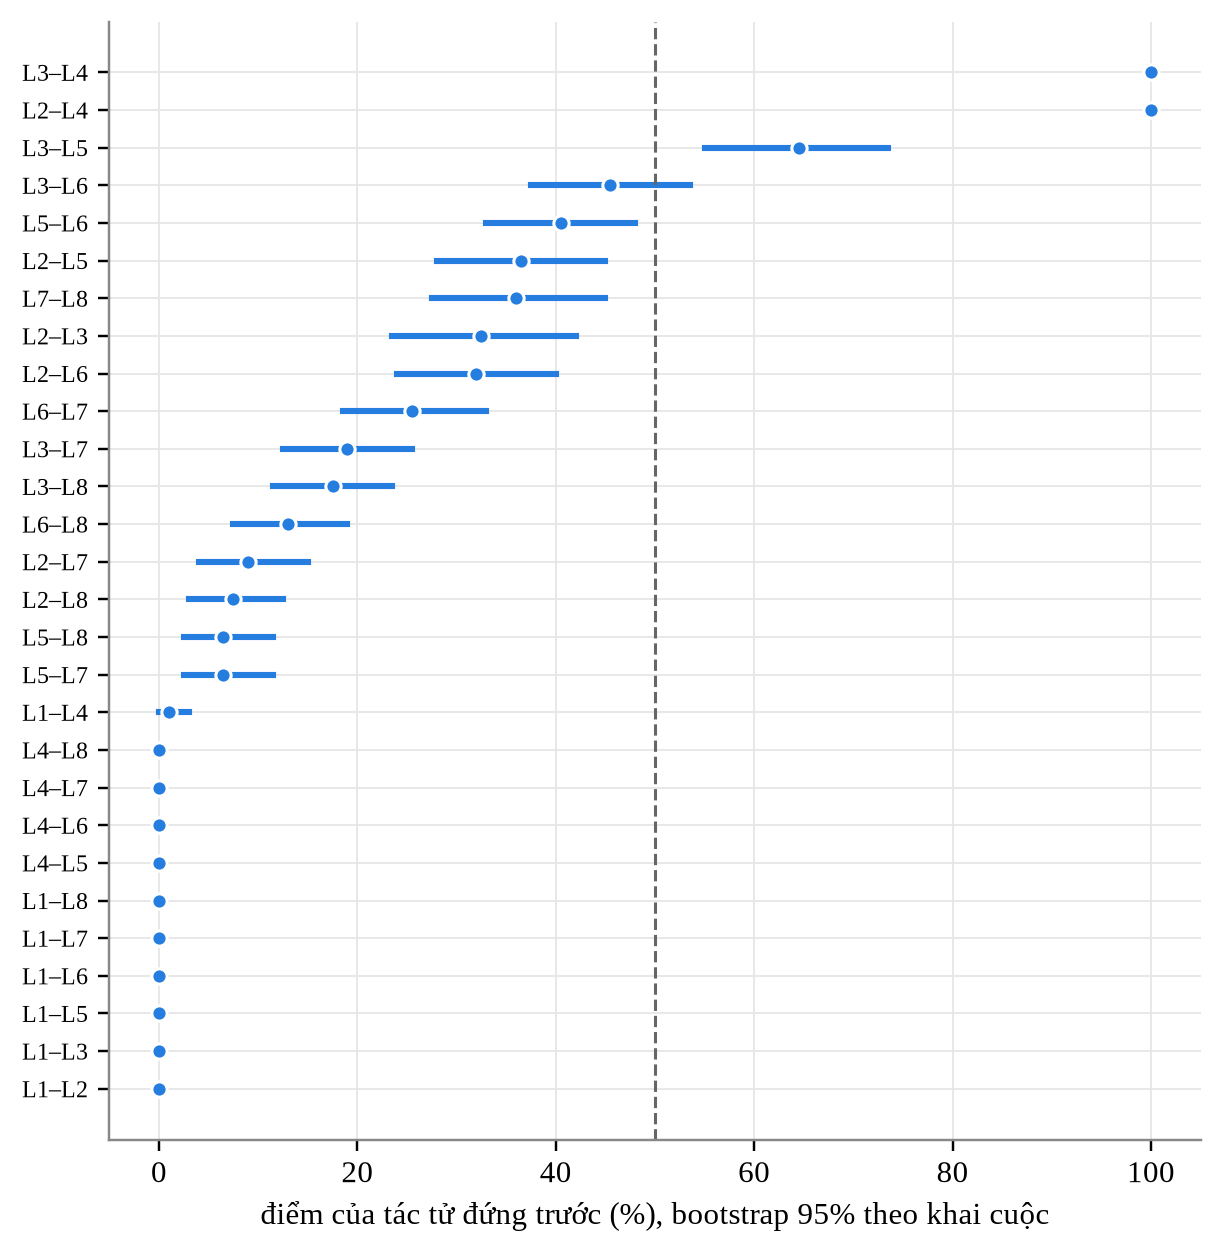
\includegraphics[width=0.92\linewidth]{chuyen-sau/hinh/tk-khoang.png}
  \caption{Điểm và khoảng bootstrap 95\% theo khai cuộc của 28 cặp. Cặp toàn thắng cho khoảng suy biến.}
  \label{fig:cs-tk-khoang}
\end{figure}
Cột ``Khi X'' và ``Khi O'' cho thấy lợi thế đi trước ngay trong cặp: giữa L6 và L7, L6 đạt $47\%$ khi cầm X nhưng chỉ
$4\%$ khi cầm O. Do đó mọi so sánh không đổi màu sẽ lệch nghiêm trọng.

\subsection{Độ nhạy của Bradley-Terry}
\begin{table}[H]
  \centering
  \small
  \caption{Điểm Bradley-Terry theo số ván hoà ảo mỗi cặp}
  \label{tab:cs-tk-prior}
  \begin{tabular}{lrrrrr}
    \toprule
    Tác tử & 0,1 & 0,5 & 1,0 & 2,0 & 5,0 \\
    \midrule
    L1 Random & -605 & -290 & -128 & 43 & 270 \\
    L2 Rule & 1209 & 1126 & 1089 & 1053 & 1013 \\
    L3 AlphaBeta & 1353 & 1269 & 1229 & 1189 & 1139 \\
    L4 MCTS & 142 & 336 & 415 & 492 & 592 \\
    L5 PolicySL & 1264 & 1180 & 1142 & 1105 & 1060 \\
    L6 PolicyRL & 1362 & 1278 & 1238 & 1198 & 1147 \\
    L7 PUCT & 1597 & 1510 & 1467 & 1421 & 1355 \\
    L8 AlphaZero & 1678 & 1590 & 1546 & 1498 & 1425 \\
    \bottomrule
  \end{tabular}
\end{table}

Khi số ván ảo mỗi cặp tăng từ $0{,}1$ lên 5, điểm L1 đổi từ khoảng $-600$ lên $270$ và khoảng cách giữa L8 và L2 thu
hẹp, nhưng \emph{thứ tự} tám tác tử không đổi. Vì vậy báo cáo diễn giải thứ hạng, còn chênh lệch Elo tuyệt đối chỉ có
nghĩa với tiên nghiệm cố định (1 ván).

\begin{table}[H]
  \centering
  \footnotesize
  \caption{Elo tuần tự phụ thuộc thứ tự ván; Bradley-Terry thì không}
  \label{tab:cs-tk-elo}
  \begin{tabular}{lrrrrr}
    \toprule
    Tác tử & B-T & Elo theo log & K=16 (200 hoán vị) & K=32 & Khoảng K=32 \\
    \midrule
    L1 Random & -128 & 225 & 218 $\pm$ 7 & 42 $\pm$ 10 & 19--68 \\
    L2 Rule & 1089 & 705 & 1013 $\pm$ 29 & 1046 $\pm$ 47 & 908--1174 \\
    L3 AlphaBeta & 1229 & 1011 & 1151 $\pm$ 30 & 1189 $\pm$ 48 & 1039--1312 \\
    L4 MCTS & 415 & 533 & 546 $\pm$ 9 & 472 $\pm$ 12 & 435--492 \\
    L5 PolicySL & 1142 & 1001 & 1064 $\pm$ 29 & 1101 $\pm$ 44 & 959--1249 \\
    L6 PolicyRL & 1238 & 1303 & 1159 $\pm$ 30 & 1196 $\pm$ 43 & 1082--1336 \\
    L7 PUCT & 1467 & 1504 & 1388 $\pm$ 29 & 1436 $\pm$ 41 & 1332--1543 \\
    L8 AlphaZero & 1546 & 1718 & 1461 $\pm$ 27 & 1518 $\pm$ 41 & 1411--1652 \\
    \bottomrule
  \end{tabular}
\end{table}

Elo tuần tự áp theo thứ tự ván trong log cho L8 khoảng 1\,718 và L6 cao hơn L3 gần 300 điểm, trong khi Bradley-Terry
cho L6 và L3 gần nhau, đúng với kết quả trực tiếp. Nguyên nhân: log chạy lần lượt từng cặp, các cặp cuối có ảnh hưởng
lớn nhất đến Elo tuần tự. Xáo trộn thứ tự 200 lần, độ lệch chuẩn khoảng 30 điểm với $K=16$ và 45 điểm với $K=32$, và
khoảng cực trị của một tác tử có thể rộng trên 200 điểm. Đây là lý do \texttt{stats.json} (Elo tuần tự) không được dùng
làm số báo cáo.

\subsection{Cần bao nhiêu khai cuộc}
\begin{table}[H]
  \centering
  \footnotesize
  \caption{Độ rộng khoảng bootstrap 95\% của điểm Bradley-Terry theo số khai cuộc}
  \label{tab:cs-tk-hoitu}
  \begin{tabular}{rrrrrrrrrr}
    \toprule
    Khai cuộc & Ván/cặp & L1 & L2 & L3 & L4 & L5 & L6 & L7 & L8 \\
    \midrule
    5 & 10 & 62 & 168 & 130 & 42 & 116 & 146 & 155 & 158 \\
    10 & 20 & 68 & 137 & 106 & 41 & 101 & 107 & 134 & 142 \\
    20 & 40 & 85 & 106 & 75 & 35 & 82 & 93 & 99 & 107 \\
    30 & 60 & 90 & 89 & 63 & 31 & 63 & 76 & 87 & 88 \\
    40 & 80 & 90 & 79 & 56 & 29 & 58 & 65 & 82 & 68 \\
    50 & 100 & 106 & 73 & 52 & 30 & 55 & 61 & 71 & 73 \\
    \bottomrule
  \end{tabular}
\end{table}

\begin{figure}[H]
  \centering
  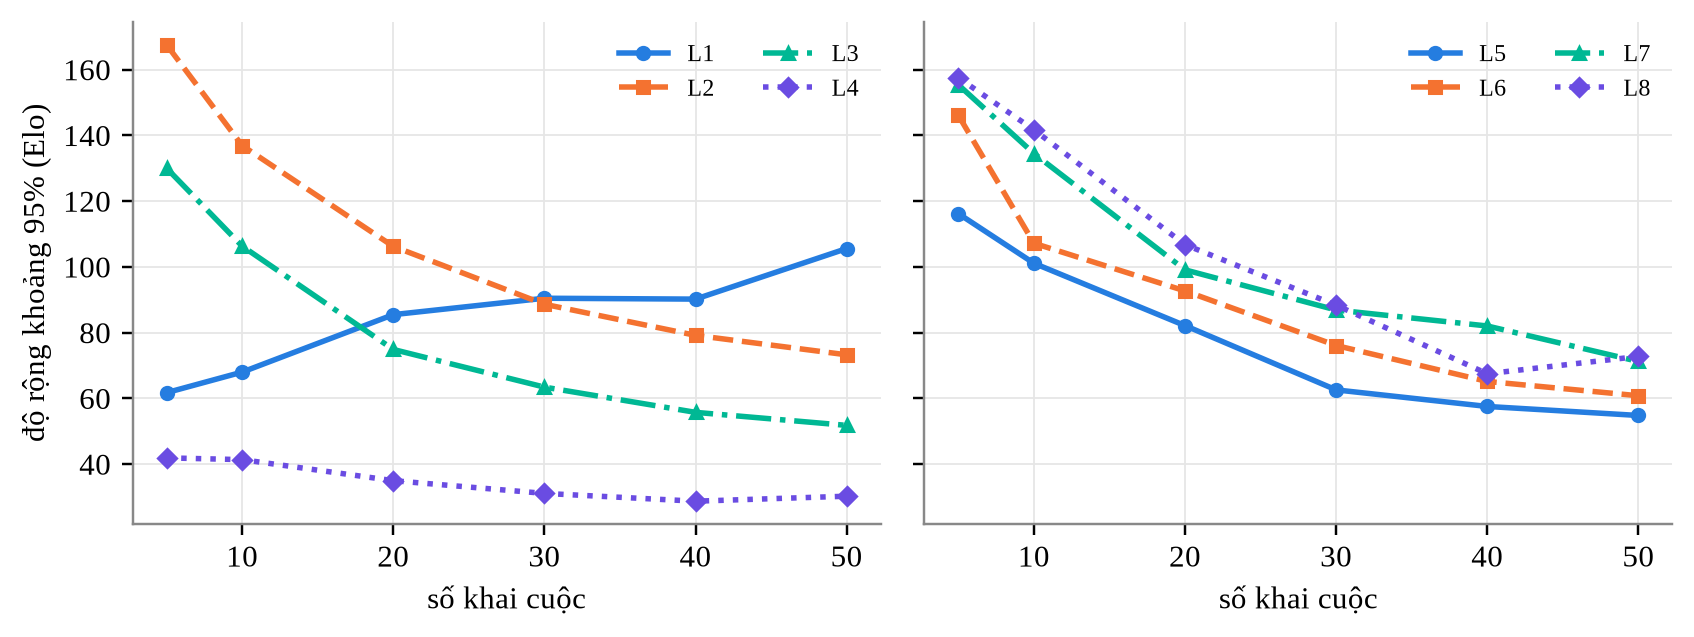
\includegraphics[width=\linewidth]{chuyen-sau/hinh/tk-hoi-tu.png}
  \caption{Độ rộng khoảng 95\% của điểm Bradley-Terry theo số khai cuộc (bootstrap 400 lần).}
  \label{fig:cs-tk-hoi-tu}
\end{figure}
Từ 5 lên 50 khai cuộc, khoảng tin cậy của các tác tử giữa bảng thu hẹp hơn một nửa, gần với tốc độ $1/\sqrt n$. Ở 50
khai cuộc, khoảng còn rộng cỡ 30--105 điểm; để giảm một nửa nữa cần khoảng bốn lần số khai cuộc.

\subsection{Mức khớp của mô hình Bradley-Terry}
\begin{figure}[H]
  \centering
  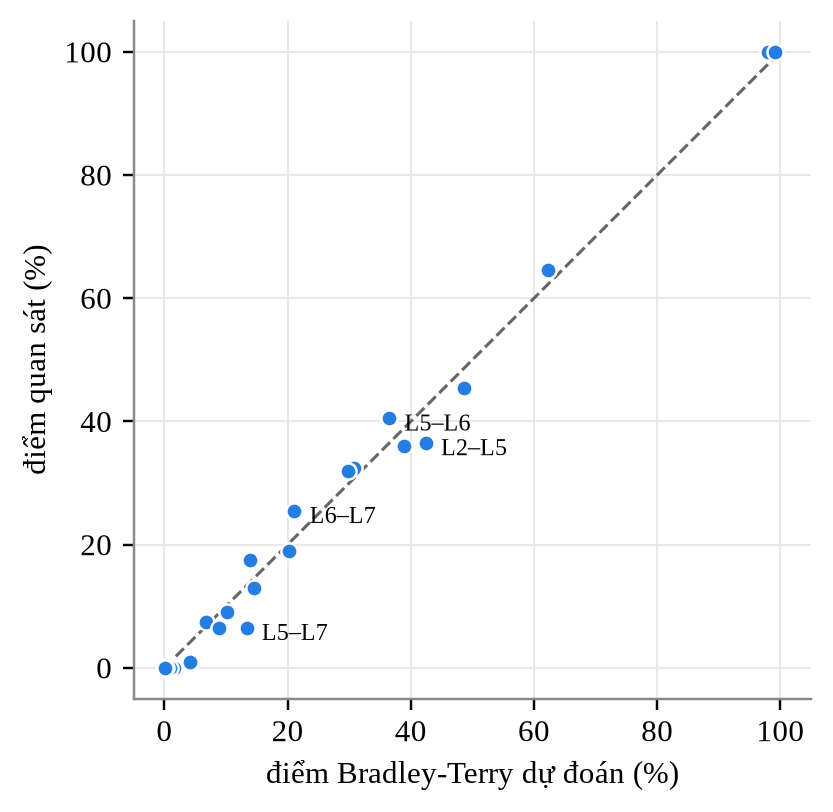
\includegraphics[width=0.55\linewidth]{chuyen-sau/hinh/tk-phan-du.png}
  \caption{Điểm quan sát so với điểm Bradley-Terry dự đoán cho 28 cặp.}
  \label{fig:cs-tk-phan-du}
\end{figure}
\begin{table}[H]
  \centering
  \small
  \caption{Mười cặp lệch nhiều nhất so với mô hình Bradley-Terry (điểm phần trăm)}
  \label{tab:cs-tk-phandu}
  \begin{tabular}{lrrr}
    \toprule
    Cặp & Quan sát & Mô hình & Phần dư \\
    \midrule
    L5--L7 & 6,5 & 13,3 & -6,8 \\
    L2--L5 & 36,5 & 42,4 & -5,9 \\
    L6--L7 & 25,5 & 21,1 & 4,4 \\
    L5--L6 & 40,5 & 36,5 & 4,0 \\
    L3--L8 & 17,5 & 13,9 & 3,6 \\
    L3--L6 & 45,5 & 48,7 & -3,2 \\
    L1--L4 & 1,0 & 4,2 & -3,2 \\
    L7--L8 & 36,0 & 38,9 & -2,9 \\
    L5--L8 & 6,5 & 8,9 & -2,4 \\
    L2--L6 & 32,0 & 29,8 & 2,2 \\
    \bottomrule
  \end{tabular}
\end{table}

Sai số căn trung bình bình phương giữa dự đoán và quan sát chỉ khoảng $2{,}6$ điểm phần trăm, và không có bộ ba nào tạo
vòng tròn thắng (A thắng B, B thắng C, C thắng A). Mô hình một chiều mô tả giải này tốt. Cặp lệch nhất là L5--L7: L5 đạt
$6{,}5\%$ trong khi mô hình dự đoán $13{,}3\%$; L7 dùng cùng mạng với L5 nên khai thác điểm yếu của chính chính sách đó
mạnh hơn mức một thang sức mạnh chung dự đoán.

\subsection{Cỡ mẫu cần thiết}
\begin{table}[H]
  \centering
  \small
  \caption{Số ván độc lập cần để phát hiện chênh lệch ($\alpha = 0{,}05$ hai phía)}
  \label{tab:cs-tk-luc}
  \begin{tabular}{rrrr}
    \toprule
    Điểm thật & Chênh Elo & Lực 80\% & Lực 90\% \\
    \midrule
    0,52 & 14 & 4.904 & 6.563 \\
    0,55 & 35 & 783 & 1.047 \\
    0,60 & 70 & 194 & 259 \\
    0,65 & 108 & 85 & 113 \\
    0,75 & 191 & 29 & 38 \\
    \bottomrule
  \end{tabular}
\end{table}

Với 100 ván mỗi cặp, đề tài đủ lực để phát hiện chênh lệch từ khoảng $65\%$ (hơn 100 Elo). Chênh lệch cỡ $55\%$ (35 Elo)
cần gần 800 ván độc lập; vì tác tử tất định chỉ cho một ván mỗi cặp khai cuộc--màu, con số đó đòi bộ khai cuộc lớn hơn
nhiều.

\subsection{Khai cuộc}
Điểm của X trung bình trên 50 khai cuộc dùng trong RR8 là $57{,}1\%$, dao động từ khoảng $47\%$ đến $69\%$ giữa các khai
cuộc (Bảng~\ref{tab:cs-tk-khaicuoc}). Số quân khai cuộc (2, 3 hay 4) không cho khác biệt đáng kể (59, 55 và 59\%). Mỗi
khai cuộc có 56 ván nên độ dao động này một phần là nhiễu mẫu; chơi đổi màu loại bỏ lợi thế khai cuộc khỏi so sánh
giữa hai tác tử.
\par{\footnotesize
\renewcommand{\arraystretch}{0.95}
\begin{longtable}{rlrrrr}
  \caption{Kết quả theo từng khai cuộc giữ riêng được dùng trong RR8}\label{tab:cs-tk-khaicuoc}\\
    \toprule
    Mã & Các nước & Ván & Điểm X (\%) & Hoà & Độ dài TB \\
    \midrule
  \endfirsthead
    \toprule
    Mã & Các nước & Ván & Điểm X (\%) & Hoà & Độ dài TB \\
    \midrule
  \endhead
    \bottomrule
  \endfoot
    0 & H6 E4 H7 & 56 & 51,8 & 0 & 19,2 \\
    1 & F4 H5 D6 D8 & 56 & 65,2 & 1 & 21,9 \\
    2 & D8 H5 & 56 & 55,4 & 0 & 20,2 \\
    3 & G6 E6 & 56 & 56,2 & 1 & 22,6 \\
    4 & D8 G7 F6 F8 & 56 & 68,8 & 1 & 24,8 \\
    5 & G7 G8 & 56 & 59,8 & 1 & 24,1 \\
    6 & G5 E7 E6 & 56 & 59,8 & 1 & 21,8 \\
    7 & E4 G6 H5 & 56 & 52,7 & 1 & 23,9 \\
    8 & D5 H6 & 56 & 65,2 & 1 & 21,3 \\
    9 & D6 H8 H6 H7 & 56 & 52,7 & 1 & 22,7 \\
    10 & F6 H7 H8 & 56 & 55,4 & 4 & 27,4 \\
    11 & H6 G6 F4 F8 & 56 & 60,7 & 0 & 20,0 \\
    12 & D4 D7 H4 H7 & 56 & 58,0 & 1 & 23,0 \\
    13 & H7 E4 F7 E5 & 56 & 60,7 & 0 & 20,9 \\
    14 & F7 F4 G6 D8 & 56 & 60,7 & 2 & 25,4 \\
    15 & F8 G7 G8 & 56 & 58,0 & 1 & 23,5 \\
    16 & G4 D7 E8 & 56 & 52,7 & 1 & 23,5 \\
    17 & G7 D6 F6 & 56 & 50,9 & 1 & 21,1 \\
    18 & G8 H8 G4 G5 & 56 & 55,4 & 2 & 24,6 \\
    19 & G5 D5 D6 & 56 & 54,5 & 1 & 23,7 \\
    20 & E7 E5 F6 H5 & 56 & 60,7 & 4 & 26,3 \\
    21 & E6 G6 H8 & 56 & 57,1 & 4 & 29,4 \\
    22 & D8 G6 G5 G8 & 56 & 50,9 & 3 & 26,5 \\
    23 & D4 F6 & 56 & 54,5 & 3 & 25,9 \\
    24 & H8 H7 E4 D8 & 56 & 65,2 & 1 & 22,7 \\
    25 & D6 H4 H8 F6 & 56 & 54,5 & 1 & 26,0 \\
    26 & H4 H6 F5 F4 & 56 & 56,2 & 3 & 28,3 \\
    27 & H4 H8 & 56 & 66,1 & 0 & 19,5 \\
    28 & G7 E4 D8 & 56 & 52,7 & 1 & 18,9 \\
    29 & H7 H6 & 56 & 63,4 & 1 & 22,6 \\
    30 & D4 F7 E4 H4 & 56 & 52,7 & 3 & 26,1 \\
    31 & D5 D8 E7 & 56 & 51,8 & 0 & 22,4 \\
    32 & D6 G5 E4 & 56 & 58,9 & 0 & 20,4 \\
    33 & H5 D4 F7 H6 & 56 & 67,0 & 1 & 22,0 \\
    34 & H8 H5 D8 & 56 & 47,3 & 1 & 21,8 \\
    35 & H8 G5 & 56 & 55,4 & 2 & 22,4 \\
    36 & E6 D8 & 56 & 58,0 & 1 & 23,1 \\
    37 & D7 D5 G4 & 56 & 52,7 & 1 & 23,7 \\
    38 & F4 D7 H7 & 56 & 63,4 & 1 & 20,9 \\
    39 & E5 G8 H7 D4 & 56 & 52,7 & 3 & 27,8 \\
    40 & H5 F7 & 56 & 56,2 & 1 & 22,9 \\
    41 & H6 D8 & 56 & 59,8 & 1 & 22,4 \\
    42 & F7 G6 G8 F4 & 56 & 60,7 & 2 & 23,2 \\
    43 & H5 F7 F5 & 56 & 50,0 & 0 & 21,1 \\
    44 & D8 H4 H5 F6 & 56 & 50,0 & 2 & 26,6 \\
    45 & H7 D5 F5 & 56 & 50,9 & 1 & 23,3 \\
    46 & H5 D5 E5 & 56 & 53,6 & 0 & 20,9 \\
    47 & H5 H6 G6 H4 & 56 & 64,3 & 2 & 25,9 \\
    48 & G7 F5 E8 & 56 & 60,7 & 2 & 25,2 \\
    49 & F5 E4 D6 & 56 & 55,4 & 2 & 26,6 \\
\end{longtable}
}


\subsection{Độ dài ván và phân bố nước đi}
\begin{figure}[H]
  \centering
  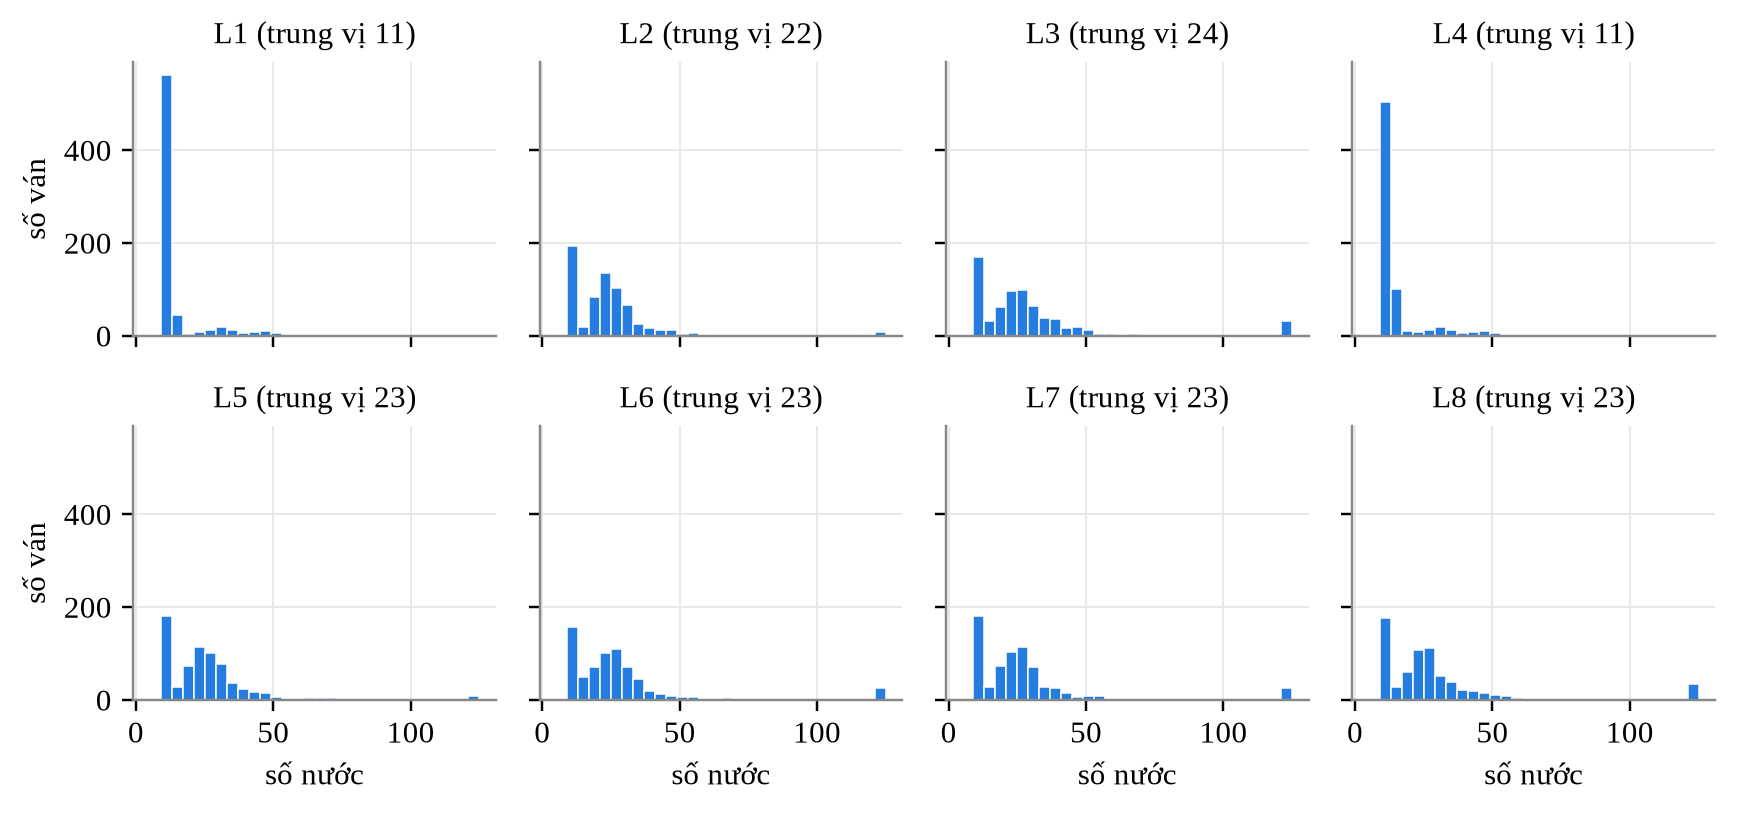
\includegraphics[width=\linewidth]{chuyen-sau/hinh/van-do-dai.png}
  \caption{Phân bố độ dài các ván có tác tử đó tham gia.}
  \label{fig:cs-van-do-dai}
\end{figure}
\begin{figure}[H]
  \centering
  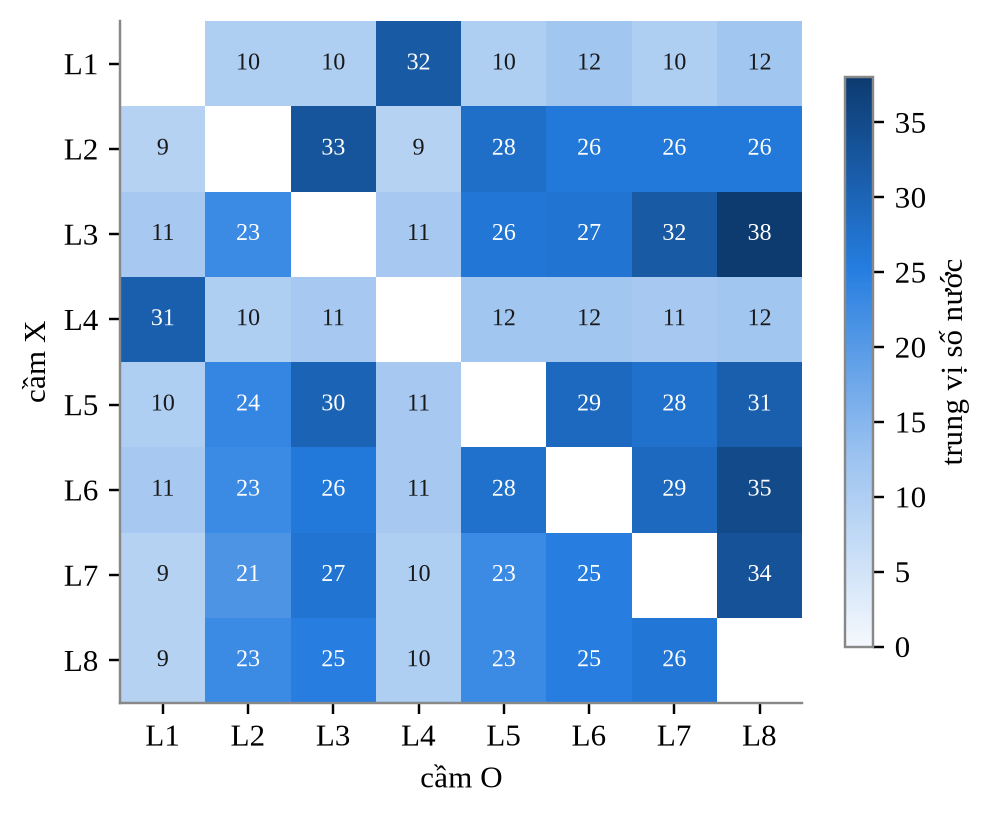
\includegraphics[width=0.66\linewidth]{chuyen-sau/hinh/van-do-dai-ma-tran.png}
  \caption{Trung vị độ dài ván theo cặp (hàng cầm X, cột cầm O).}
  \label{fig:cs-van-do-dai-mt}
\end{figure}
Các ván dài nhất thuộc về cặp ngang sức giữa các cấp có kiến thức; trừ cặp L1--L4, ván giữa L1 hoặc L4 với một cấp
có kiến thức thường kết thúc quanh nước 10--12, tức bên mạnh thắng bằng đòn đầu tiên.

\begin{figure}[H]
  \centering
  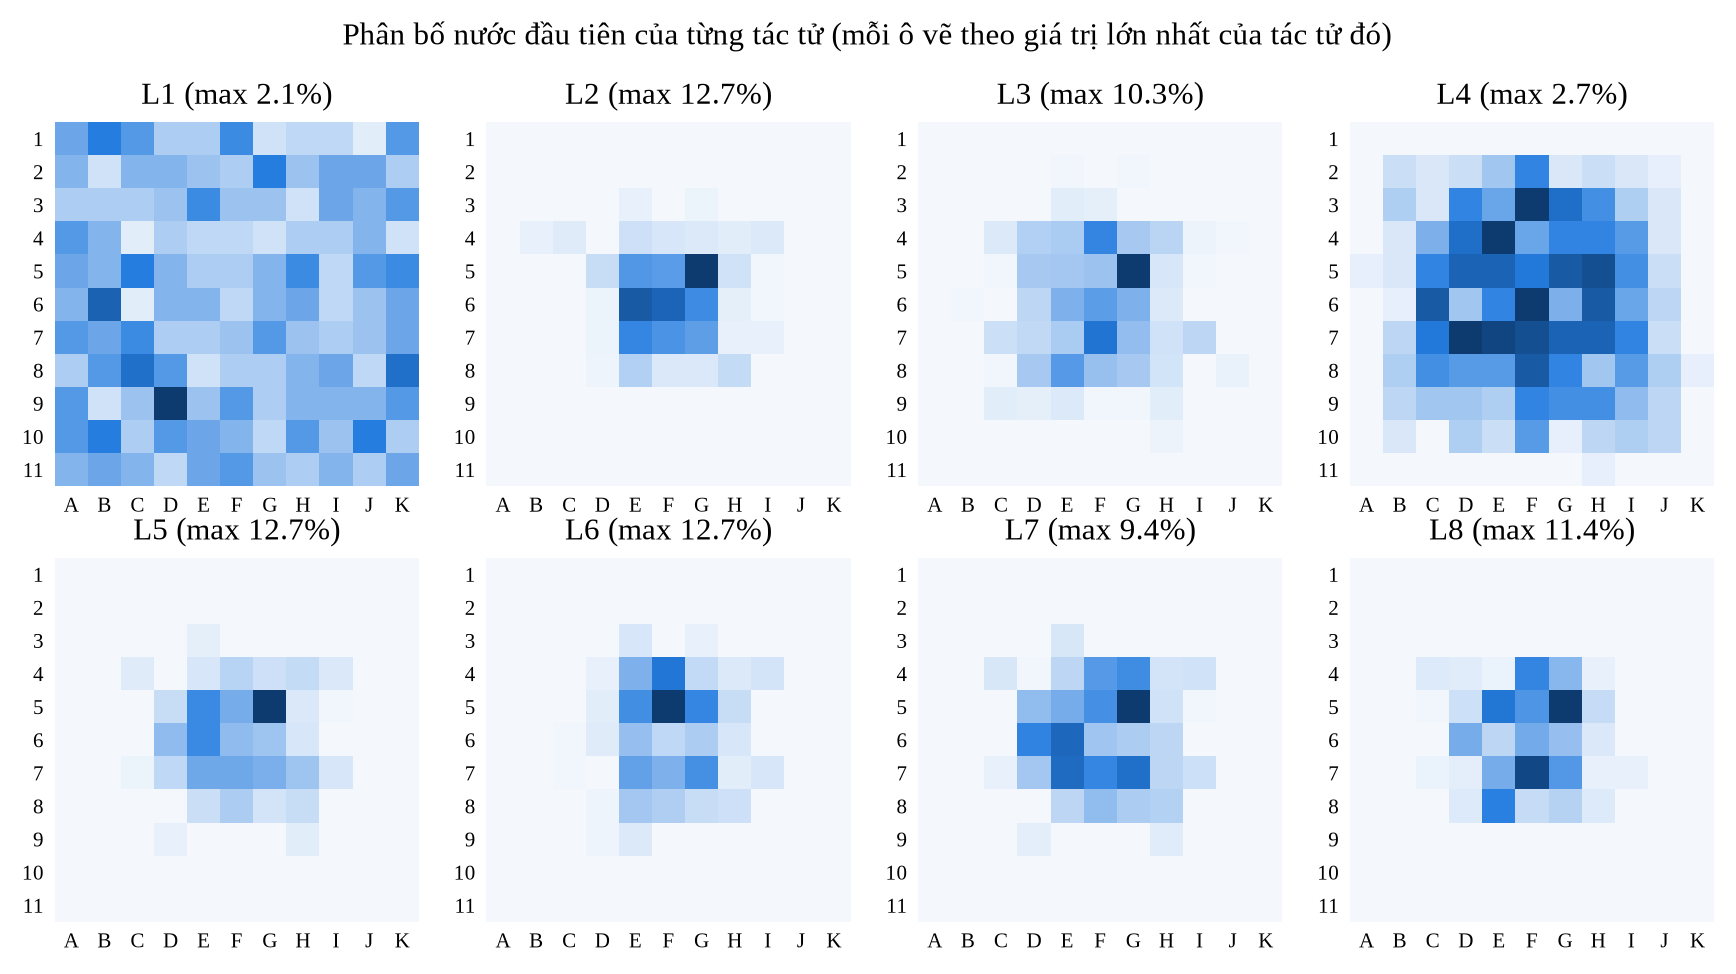
\includegraphics[width=\linewidth]{chuyen-sau/hinh/van-nuoc-dau.png}
  \caption{Phân bố nước đầu tiên (sau khai cuộc) của từng tác tử.}
  \label{fig:cs-van-nuoc-dau}
\end{figure}
\begin{figure}[H]
  \centering
  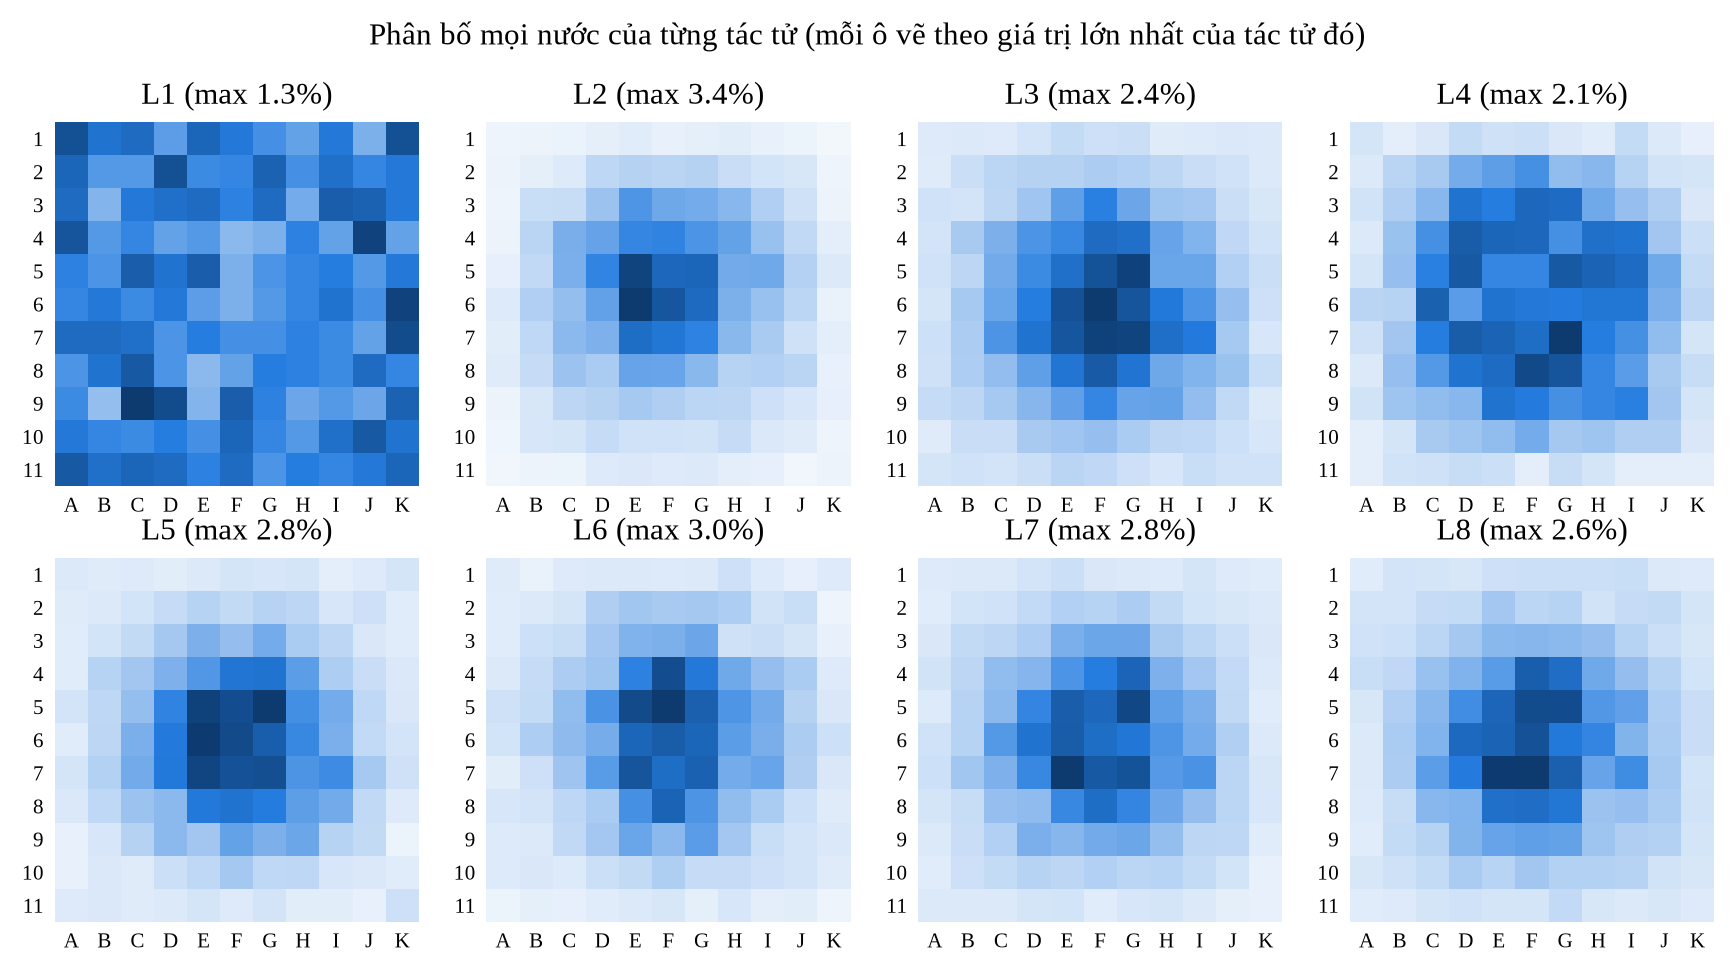
\includegraphics[width=\linewidth]{chuyen-sau/hinh/van-moi-nuoc.png}
  \caption{Phân bố mọi nước đi của từng tác tử.}
  \label{fig:cs-van-moi-nuoc}
\end{figure}
\begin{table}[H]
  \centering
  \small
  \caption{Phân bố không gian của nước đi}
  \label{tab:cs-tk-khonggian}
  \begin{tabular}{lrrrr}
    \toprule
    Tác tử & Cách nước trước & Kề nước trước (\%) & Vùng 5$\times$5 (\%) & Ô biên (\%) \\
    \midrule
    L1 Random & 4,41 & 6,1 & 17,9 & 35,5 \\
    L2 Rule & 2,65 & 32,8 & 49,5 & 6,6 \\
    L3 AlphaBeta & 3,03 & 27,9 & 44,0 & 12,4 \\
    L4 MCTS & 3,76 & 11,0 & 38,4 & 10,0 \\
    L5 PolicySL & 2,96 & 26,4 & 49,8 & 10,0 \\
    L6 PolicyRL & 2,77 & 32,6 & 48,4 & 9,9 \\
    L7 PUCT & 2,90 & 29,2 & 46,4 & 10,8 \\
    L8 AlphaZero & 2,74 & 33,7 & 45,3 & 12,4 \\
    \bottomrule
  \end{tabular}
  \par\smallskip\parbox{.95\linewidth}{\footnotesize Khoảng cách Chebyshev tới nước vừa đi của đối thủ.}
\end{table}

Phân bố nước đi phản ánh cách tìm: ngẫu nhiên phủ đều bàn; MCTS rollout trải rộng và chỉ $11\%$ nước kề nước vừa đi
của đối thủ; các tác tử còn lại tập trung ở giữa và chơi sát. L8 kề nhiều nhất ($33{,}7\%$).

\subsection{Thời gian theo giai đoạn}
\begin{figure}[H]
  \centering
  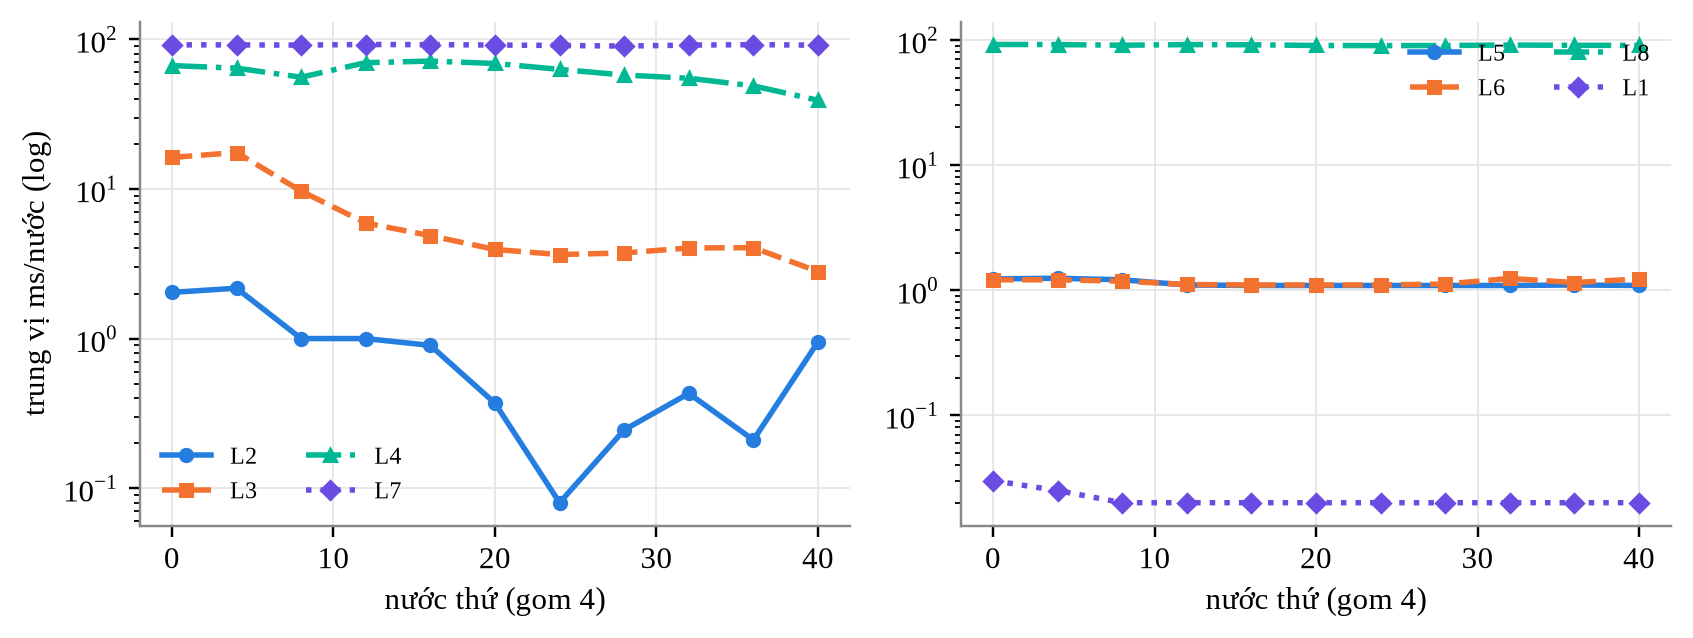
\includegraphics[width=\linewidth]{chuyen-sau/hinh/van-thoi-gian.png}
  \caption{Trung vị thời gian mỗi nước theo giai đoạn ván (thang log); chỉ vẽ nhóm có từ 30 nước.}
  \label{fig:cs-van-thoi-gian}
\end{figure}
\begin{table}[H]
  \centering
  \small
  \caption{Trung vị thời gian mỗi nước (ms) theo giai đoạn trong RR8 giữ riêng}
  \label{tab:cs-tk-thoigian}
  \begin{tabular}{lrrrrrr}
    \toprule
    Tác tử & từ 0 & từ 8 & từ 16 & từ 24 & từ 32 & từ 40 \\
    \midrule
    L1 Random & 0,0 & 0,0 & 0,0 & 0,0 & 0,0 & 0,0 \\
    L2 Rule & 2,0 & 1,0 & 0,9 & 0,1 & 0,4 & 0,9 \\
    L3 AlphaBeta & 16,2 & 9,7 & 4,9 & 3,6 & 4,0 & 2,8 \\
    L4 MCTS & 66,7 & 55,8 & 71,5 & 63,0 & 54,9 & 39,1 \\
    L5 PolicySL & 1,2 & 1,2 & 1,1 & 1,1 & 1,1 & 1,1 \\
    L6 PolicyRL & 1,2 & 1,2 & 1,1 & 1,1 & 1,2 & 1,2 \\
    L7 PUCT & 91,8 & 91,4 & 92,0 & 90,9 & 91,4 & 91,3 \\
    L8 AlphaZero & 92,0 & 90,7 & 91,5 & 90,1 & 91,1 & 90,4 \\
    \bottomrule
  \end{tabular}
\end{table}

Với ngân sách số mô phỏng cố định, L7 và L8 tốn gần như không đổi theo giai đoạn. Alpha-Beta nhanh dần khi bàn đông vì
nước bắt buộc thu hẹp cây; L2 rẻ nhất ở trung cuộc muộn khi các luật đầu khớp sớm.
